\documentclass[polish, 11pt]{article}

\usepackage[a4paper, margin=25mm]{geometry}
\usepackage{babel}
\usepackage{polski}
\usepackage[utf8]{inputenc}
\usepackage[T1]{fontenc}
\usepackage{lmodern}
\usepackage{graphicx}
\usepackage{pdfpages}
\usepackage{listings}
\usepackage{float}
\usepackage{xcolor}
\usepackage{gasasm}
\usepackage{hyperref}
\hypersetup{
    colorlinks=true,
    linkcolor=blue,
    filecolor=magenta,      
    urlcolor=cyan,
}
\graphicspath{ {images/} }
\lstset{language=[GAS]Assembler}


\begin{document}
	\begin{flushright}
		Wrocław, \ \today\\
	\end{flushright}
	Emilia Pawlaszek, 241279\\
	Łukasz Szumilas, 236068\\
	
    \vspace{0,3cm}
    PN TN 13:15
	
	\vspace{2cm}
	\begin{center}
	\begin{Large}
	\emph{Sprawozdanie z projektu przedmiotu „Architektura Komputerów 2”}
	\end{Large}
	\end{center}
	\begin{center}
    Rok akad. 2018/2019, kierunek: INF
    \end{center}
	\begin{flushright}
	Prowadzący:\\
	dr inż. Dominik Żelazny
	\vspace{1cm}
	\end{flushright}
	\vfill
	
\newpage
\tableofcontents

\newpage
\section{Założenia projektu}
Celem projektu jest stworzenie systemu pobierającego dane pogodowe i przesyłającego ich na urządzenie odbierające dane. System bez ingerencji człowieka ma być w stanie mierzyć temperaturę, wilgotność powietrza, ciśnienie atmosferyczne i natężenie światła.\\
Dodatkowo za pomocą modułu wifi i przeglądarki układ łączy się z odbiorcą i automatycznie przesyła dane. 

\vspace{1cm}
\section{Wykorzystane narzędzia}
System powstał w oparciu o model Arduino Uno, wraz z rozszerzeniami:\\
\begin{itemize}
    \item DHT11 – czujnik wilgotnosci i temperatury,
    \item BH1750 – czujnik natezenia swiatla,
    \item BMP180 – czujnik ciśnienia i temperatury,
    \item ESP8266 – modul wifi.
\end{itemize}
Dodatkowo:
\begin{itemize}
    \item Przewód USB
    \item Płytka stykowa
    \item Rezystory
    \item Przewody, kable
\end{itemize}

\vspace{1cm}
\section{Realizacja}
Realizacja rozpoczęła się od poznania teoretycznych zagadnień dotyczących czujników: ich wejść, wyjść, sposobu działania i przesyłu danych na platformę Arduino. 

\subsection{Czujnik DHT11}
Czujnik ten odpowiada za pokazywanie pomiarów wilgotności względnej. Wartości te są z przedziału 0-1 i nie posiadają jednostki, więc w projekcie grupa przedstawiała je jako procent ciśnienia cząstkowego pary wodnej zawartej w powietrzu do ciśnienia nasycenia nad płaską powierzchnią czystej wody, gdzie: 0\% to powietrze całkowicie suche, 100\% maksymalnie wilgotne. Sensor ten posiada także wbudowany termometr w zakresie 0-50 stopni Celcjusza, jednak nie został on użyty w projekcie. 

\pagebreak
\begin{center}Czujnik ten składa się z następujących wejść:\end{center} 
\begin{figure}[H]
    \centering
    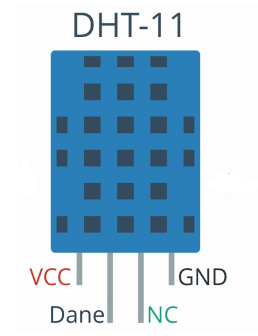
\includegraphics[scale=0.6]{dht11.png}
\caption{Czujnik DHT11 i jego wejścia}
\end{figure}
\textbf{\textit{VCC}} podpina się do zasilania 5V, \textbf{\textit{GND}} oznacza Ground. Jest to masa, która służy do wyrównania potencjałów w układzie. Drugi pin z danymi był podłączony do jednego wejścia na Arduino \textit{PWM} (Pulse Width Modulation), co oznacza modulację szerokości impulsu. Z tak pobieranych danych jest mierzony procent czasu, przez jaki sygnał ma potencjał wysoki i kiedy rzeczywiście informacje o wilgotności są przekazywane na mikrokontroler. Oprócz tego przy wyprowadzaniu danych trzeba skorzystać z rezystora pull-up, by podtrzymać (kiedy zachodzi taka potrzeba) stan wysoki i zapobiec jednocześnie stanom nieustalonym. 


\subsection{Czujnik BMP180}
W przypadku tego urządzenia powinno się zwrócić szczególną uwagę na wejście \textbf{\textit{VCC}}, które podpina się do 3.3V, gdyż tylko takie napięcie może przyjąć. 
\begin{figure}[H]
    \centering
    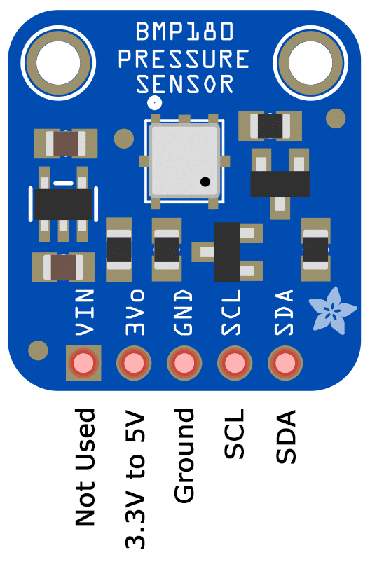
\includegraphics[scale=0.3]{bmp180.png}
\caption{Czujnik BMP180}
\end{figure}
Po drugiej stronie widać wejście \textbf{\textit{GND}}, zewnętrzne piny odpowiadają więc za to samo co piny o tej samej nazwie opisane w \textit{DHT11}. Najważniejsze to \textbf{\textit{SCL}} i \textbf{\textit{SDA}}. Należą one do dwukierunkowej, szeregowej magistrali $I^2C$, gdzie SCL odpowiada to linia zegara natomiast SDA to linia danych. Obie są na stałe podciągnięte do źródła zasilania dzięki wbudowanemu rezystorowi pull-up, przez co nie ma potrzeby dodawania do schematu kolejnego opornika. Na płytce Arduino znajdują się specjalne wejścia do komunikacji z taką magistralą o takich samych nazwach. 

\par BMP180 charakteryzuje się pomiarem ciśnienia w zakresie od 300 do 1100 hPa, co daje  możliwość określenia wysokości od +9000 do -500 metrów względem poziomu morza.
\par Czujnik, by pokazać poprawne pomiary ciśnienia, musi wpierw pobrać aktualną temperaturę, grupa więc zdecydowała na pomiar stopni Celsjusza tym sensorem zamiast \textit{DHT11}. 
W programie można także obliczać aktualną wysokość nad poziomem morza dzięki wbudowanemu algorytmowi, mając na wejście informacje o ciśnieniu nad poziomem morza. 

\subsection{Czujnik BH1750}
BH1750 to cyfrowy czujnik natężenia światła działający w zakresie 1 - 65535 lx (luks), gdzie luks określany jest jako oświetlenie wywołane przez równomiernie rozłożony strumień świetlny o wartości równej 1 lumen (lm) padający na powierzchnię $1 m^2$. 

\begin{figure}[H]
    \centering
    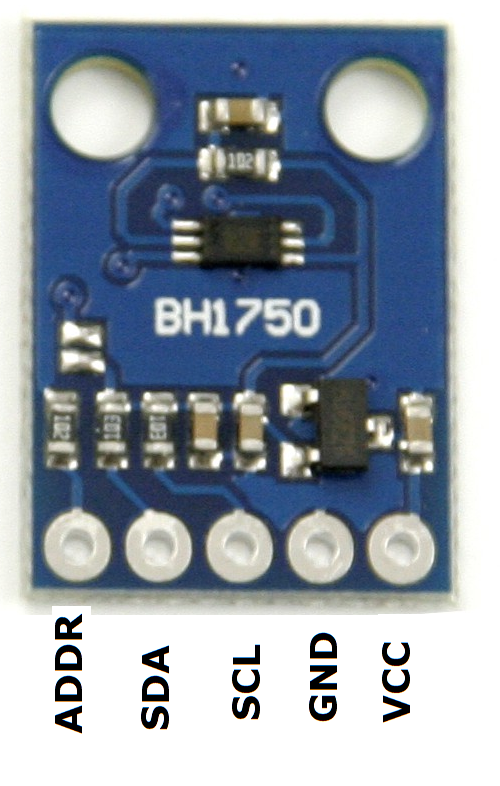
\includegraphics[scale=0.2]{BH1750.png}
\caption{Czujnik BH1750}
\end{figure}
Podobnie jak w przypadku BMP180, sensor komunikuje się poprzez interfejs $I^2C$. Można go stosować do pomiaru natężenia światła zarówno w pomieszczeniach jak i w obszarze otwartym. Wejście \textbf{\textit{ADDR}} sygnalizuje o wyborze adresu magistrali, w przypadku tego projektu nie musiało być używane. 

\subsection{Moduł WiFi ESP8266}
Urządzenie to umożliwia bezprzewodową komunikację szeregową po WiFi do Internetu. Z całej rodziny opartych na chipie ESP8266, grupa wybrała model ESP-01.Działa on w standardzie WiFI 802.11 b/g/n na częstotliwości 2,4 GHz. Zasięg samego urządzenia to 300 metrów, a możliwość podłączenia go z lokalnym routerem posiadającym dostęp do Internetu sprawia, że posiadając zewnętrzny adres IP i zarezerwowany port może komunikować się z całym światem. 
\begin{figure}[H]
    \centering
    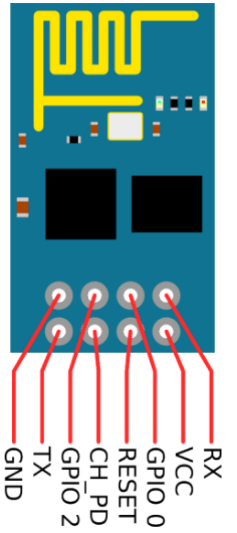
\includegraphics[scale=0.4]{esp8266.png}
\caption{Moduł WiFi ESP8266}
\end{figure}
Model ten posiada dodatkowe wyprowadzenia GPIO (\textit{ general-purpose input/output}), które odpowiadają za komunikację z np. urządzeniami peryferyjnymi, więc nie przydają się w realizacji tego projektu. Wyjście VCC wymaga zasilania na poziomie 3,3V. \textbf{\textit{RX}} i \textbf{\textit{TX}} odpowiadają kolejno za odbiór i nadawanie danych. W dołączonym kodzie widać, że w połączeniu szeregowym na Arduino za te funkcje odpowiedzialne są piny 2 i 3. W realizacji komunikacji modułu z resztą układu bardzo pomogła biblioteka \textit{WiFiEsp.h}. Zapobiegała ona bezpośredniemu przesyłaniu komend AT, które ogólnie służą do komunikacji z modemami i są dosyć nieintuicyjne. Piny \textbf{\textit{CHPD}} i \textbf{\textit{Reset}} muszą być w stanie wysokim, więc również wędrują do zasilania 3,3V. 

\section{Programowanie}
Arduino poprzez USB zostaje podłączone do komputera, gdzie za pomocą Arduino IDE można utworzyć kod programu komunikujący się z urządzeniem. 
\begin{figure}[H]
    \centering
    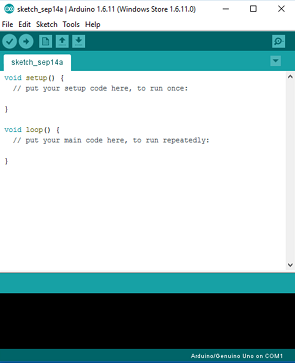
\includegraphics {arduinoide.png}
\caption{Środowisko programistyczne dla Arduino}
\end{figure}
Programy mogą być pisane w języku C/C++, jednak IDE znacznie ułatwia tworzenie kodu dzięki domyślnym bibliotekom, takim jak \textit{Wiring}. Prostsze kody składają się przeważnie z dwóch części:
\begin{itemize}
    \item setup() – funkcja wykonywana raz, na początku działania programu, wykorzystywana najczęściej do ładowania ustawień,
    \item loop() – funkcja wywoływana wielokrotnie, przez cały okres działania programu, czyli do czasu odłączenia zasilania od układu.
\end{itemize}
\par Do praktycznie każdego czujnika na stronie \textit{GitHub} \url{https://github.com/adafruit} można znaleźć bibliotekę, która pomaga w sterowaniu danymi pobieranymi przez dany sensor. Znajduje się tam ponad 1000 repozytoriów do różnych urządzeń, a przykłady kodów dołączanych wraz z biblioteką powodują, że programowanie staje się łatwe i przyjemne. 
\par Dane miejsca w kodze podczas działania programu poprzez podłączoną płytkę można podglądać dzięki monitorowaniu portu szeregowego. Pokazuje on miejsca, które podczas realizacji kodu wypisują dane poprzez komendę: \textit{Serial.print("przykładowa wiadomość")}. Dzięki temu programista może sprawdzić dane wysyłane np. poprzez czujnik DHT11, zanim będzie realizował dalszą część projektu. 
\par Nie licząc języka C++, w programie został także użyty język znaczników HTML. Ministrona została nadawana poprzez moduł WiFi do klientów, chcących połączyć się i pobrać dane z serwera. 


\vspace{1cm}
\section{Schematy połączeń}
\begin{figure}[H]
    \centering
    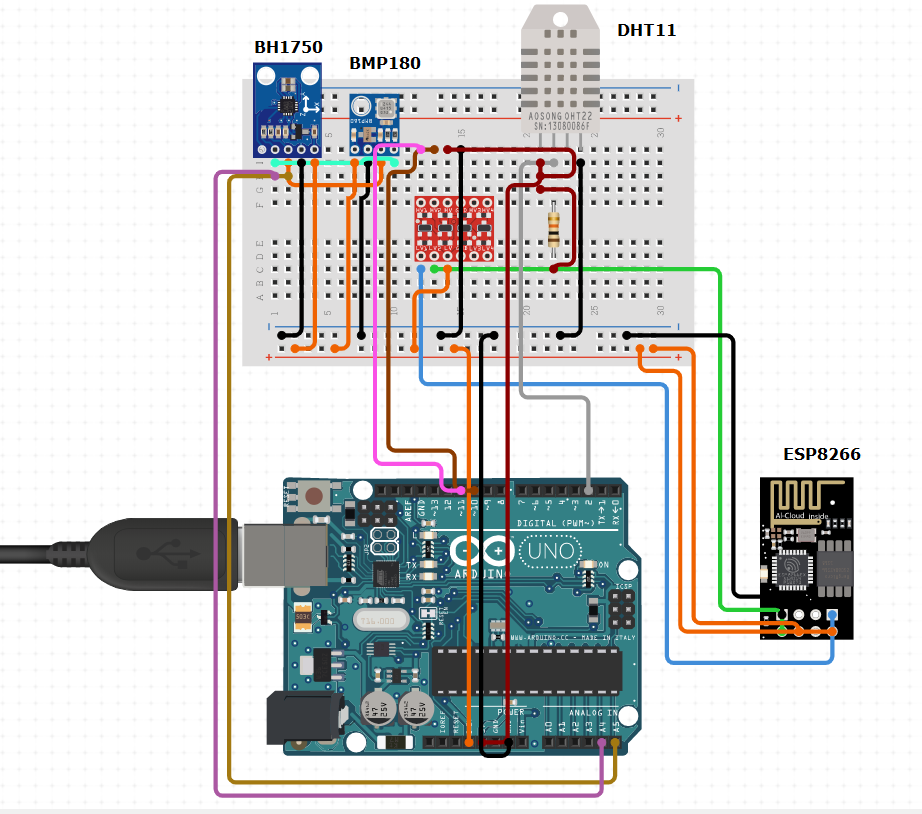
\includegraphics[scale=0.8]{schemat.png}
\caption{Schemat}
\end{figure}

\vspace{1cm}
\section{Trudności w realizacji projektu}
Grupa napotkała na trudności związane z fizycznym połączeniem niektórych części. Okazało się, że czujniki BMP180 i BH1750 posiadają piny niezlutowane z samymi płytkami, przez co grupa musiała zlutować sensory za pomocą cyny w taki sposób, by pobór danych przebiegał bez zakłóceń. Była to dobra okazja do nabycia kolejnej ciekawej umiejętności. 
\par Podpięcie wszystkich czujników do Arduino za pomocą kabli i płytki stykowej także nie należało do najłatwiejszych zadań, głównie przez mnogość kabli, co widać na zdjęciach w następnej sekcji. Bez odpowiednich narzędzi do segregacji kabli i schowania ich pod płytkę ciężko jest dostrzec, co za co odpowiada. 

\vspace{1cm}
\section{Zdjęcia systemu}
\begin{figure}[H]
    \centering
    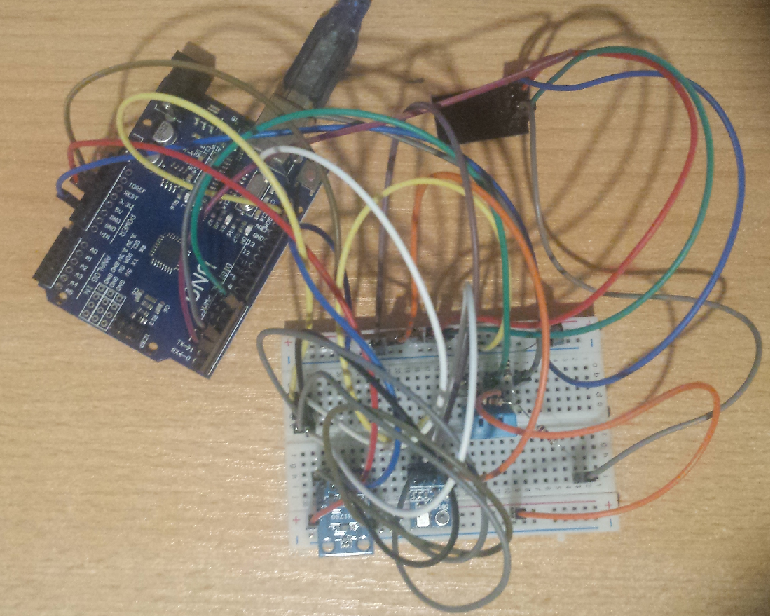
\includegraphics[scale=0.6]{all.png}
\caption{Całość systemu}
\end{figure}

\begin{figure}[H]
    \centering
    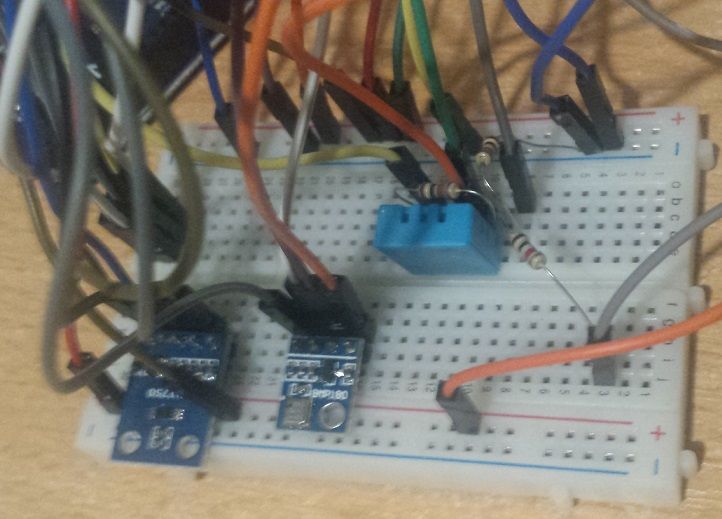
\includegraphics[scale=0.5]{modules.jpg}
\caption{Moduły}
\end{figure}

\begin{figure}[H]
    \centering
    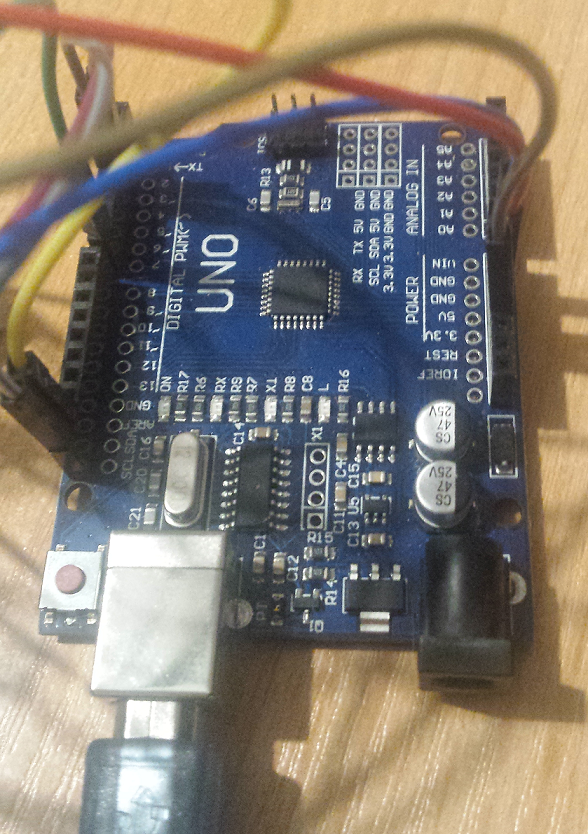
\includegraphics[scale=0.5]{arduino.png}
\caption{Arduino}
\end{figure}

\begin{figure}[H]
    \centering
    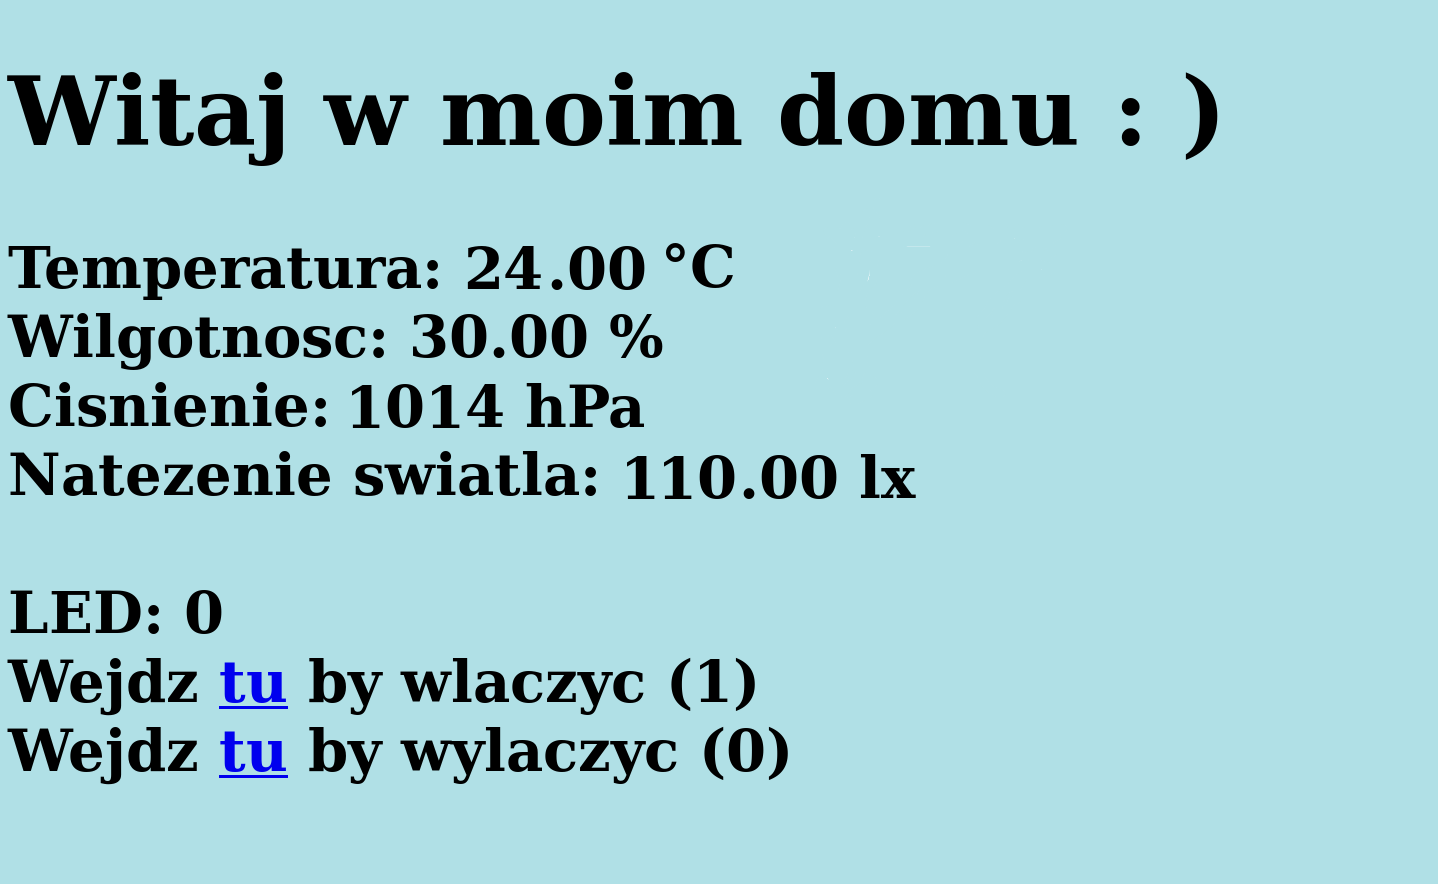
\includegraphics[scale=0.2]{view.png}
\caption{Przykładowe pomiary na stronie}
\end{figure}

\vspace{1cm}
\section{Wnioski}
Projekt stacji pogodowej grupie udało się zrealizować bez większych przeszkód. Układ działa poprawnie i zgodnie z założeniami projektu. Po umieszczeniu systemu w odpowiedniej obudowie może on służyć jako autonomiczna stacja pogodowa. 

\vspace{1cm}
\begin{thebibliography}{99}
	\addcontentsline{toc}{section}{Bibliografia}

    \bibitem{wiki} \texttt{https://pl.wikipedia.org/wiki}
    \bibitem{arduino} \texttt{https://www.arduino.cc}
\end{thebibliography}
\end{document}
